% This is "bach-ref-2009.tex" Updated january 29th 2010.
% This file should be compiled with "sig-alternate-fixed.cls" January 2010.
% It is based on the ACM style "sig-alternate.cls"
% -------------------------------------------------------------------------
% This example file demonstrates the use of the 'sig-alternate-fixed.cls'
% V2.5 LaTeX2e document class file. It is for those submitting
% articles to the Twente Student Conference on IT. Both this file as the 
% document class file are based upon ACM documents.
%
% ----------------------------------------------------------------------------------------------------------------
% This .tex file (and associated .cls) produces:
%       1) The Permission Statement
%       2) The Conference (location) Info information
%       3) The Copyright Line TSConIT
%       4) NO headers and/or footers
%
%
% Using 'sig-alternate.cls' you have control, however, from within
% the source .tex file, over both the CopyrightYear
% (defaulted to 200X) and the ACM Copyright Data
% (defaulted to X-XXXXX-XX-X/XX/XX).
% e.g.
% \CopyrightYear{2007} will cause 2007 to appear in the copyright line.
% \crdata{0-12345-67-8/90/12} will cause 0-12345-67-8/90/12 to appear in the copyright line.
%
% ---------------------------------------------------------------------------------------------------------------
% This .tex source is an example which *does* use
% the .bib file (from which the .bbl file % is produced).
% REMEMBER HOWEVER: After having produced the .bbl file,
% and prior to final submission, you *NEED* to 'insert'
% your .bbl file into your source .tex file so as to provide
% ONE 'self-contained' source file.
%

% refers to the cls file being used
\documentclass{sig-alternate-br}
\usepackage{footnote}

\begin{document}

% --- Author Metadata here --- DO NOT REMOVE OR CHANGE 
\conferenceinfo{32$^{nd}$ Twente Student Conference on IT}{Jan. 31$^{st}$, 2019, Enschede, The Netherlands.}
\CopyrightYear{2019} % Allows default copyright year (200X) to be over-ridden - IF NEED BE.
%\crdata{0-12345-67-8/90/01}  % Allows default copyright data (0-89791-88-6/97/05) to be over-ridden - IF NEED BE.
% --- End of Author Metadata ---

\title{Empirical Comparison of Automated Machine Learning Techniques for Data Streams}
% In Bachelor Referaat at University of Twente the use of a subtitle is discouraged.
% \subtitle{[Instructions]}

%
% You need the command \numberofauthors to handle the 'placement
% and alignment' of the authors beneath the title.
%
% For aesthetic reasons, we recommend 'three authors at a time'
% i.e. three 'name/affiliation blocks' be placed beneath the title.
%
% NOTE: You are NOT restricted in how many 'rows' of
% "name/affiliations" may appear. We just ask that you restrict
% the number of 'columns' to three.
%
% Because of the available 'opening page real-estate'
% we ask you to refrain from putting more than six authors
% (two rows with three columns) beneath the article title.
% More than six makes the first-page appear very cluttered indeed.
%
% Use the \alignauthor commands to handle the names
% and affiliations for an 'aesthetic maximum' of six authors.
% Add names, affiliations, addresses for
% the seventh etc. author(s) as the argument for the
% \additionalauthors command.
% These 'additional authors' will be output/set for you
% without further effort on your part as the last section in
% the body of your article BEFORE References or any Appendices.

\numberofauthors{1} %  in this sample file, there are a *total*
% of EIGHT authors. SIX appear on the 'first-page' (for formatting
% reasons) and the remaining two appear in the \additionalauthors section.
%
\author{
% You can go ahead and credit any number of authors here,
% e.g. one 'row of three' or two rows (consisting of one row of three
% and a second row of one, two or three).
%
% The command \alignauthor (no curly braces needed) should
% precede each author name, affiliation/snail-mail address and
% e-mail address. Additionally, tag each line of
% affiliation/address with \affaddr, and tag the
% e-mail address with \email.
%
% 1st. author
\alignauthor
Alexandru-Ionut Imbrea\\
       \affaddr{University of Twente}\\
       \affaddr{P.O. Box 217, 7500AE Enschede}\\
       \affaddr{The Netherlands}\\
       \email{a.imbrea@student.utwente.nl}
}

\maketitle

\begin{abstract}
Automated machine learning techniques benefited from tremendous research progress in recently. These developments and the continuous-growing demand for machine learning experts led to the development of numerous AutoML tools. However, these tools assume that the entire training dataset is available upfront and that the underlying distribution does not change over time. These assumptions do not hold in a data stream mining setting where an unbounded stream of data cannot be stored and is likely to manifest concept drift. Industry applications of machine learning on streaming data become more popular due to the increasing adoption of real-time streaming patterns in IoT, microservices architectures, web analytics, and other fields. The research summarized in this paper surveys the state-of-the-art open-source AutoML tools, applies them to data collected from streams, and measures how their performance changes over time. For comparative purposes, batch, batch incremental and instance incremental estimators are applied and compared. Moreover, a meta-learning technique for online algorithm selection based on meta-feature extraction is proposed and compared while model replacement and continual AutoML techniques are discussed. The results show that off-the-shelf AutoML tools can provide satisfactory results but in the presence of concept drift, detection or adaptation techniques have to be applied to maintain the predictive accuracy over time.
\end{abstract}

% A category with the (minimum) three required fields (NOT USED in Bachelor Referaat)
% \category{H.4}{Information Systems Applications}{Miscellaneous}
%A category including the fourth, optional field follows...
% \category{D.2.8}{Software Engineering}{Metrics}[complexity
% measures, performance measures]

\keywords{AutoML, AutoFE, Hyperparameter Optimization, Online Learning, Meta-Learning, Data Stream Mining}

\section{Introduction}
Developing machine learning models that provide constant high predictive accuracy is a difficult task that usually requires the expertise of a data scientist. Data scientists are multidisciplinary individuals possessing skills from the intersection of mathematics, computer science, and business/domain knowledge. Their job mainly consists of performing a workflow that includes, among others, the following steps: data gathering, data cleaning, feature extraction, algorithm selection, and hyperparameter optimization. The last three steps of this workflow are iterative tasks that involve fine-tuning which is usually performed by data scientists in a trial-and-error process until the desired performance is achieved. The ever-growing amount of machine learning algorithms and hyperparameters leads to an increase in the number of configurations which makes data scientists' job more laborious than ever. 

Considering the above reason and due to the lack of experts required in the industry, the field of Automated Machine Learning (Auto ML) benefited from considerable advances recently \cite{elshawi2019automated}. AutoML tools and techniques enable non-experts to achieve satisfactory results and experts to automate and optimize their tasks. Although the field of AutoML is relatively new, it consists of multiple other sub-fields such as Automated Data Clean (Auto Clean), Automated Feature Engineering (Auto FE), Hyperparameter Optimization (HPO), Neural Architecture Search (NAS), and Meta-Learning. The sub-field of Meta-Learning is concerned with solving the algorithm selection problem \cite{rice1976algorithm} applied to ML by selecting the algorithm that provides the best predictive performance for a data set. HPO techniques are used to determine the optimal set of hyperparameters for a learning algorithm, while Auto FE aims to extract and select features automatically. NAS represents the process of automating architecture engineering for artificial neural networks which already outperformed manually designed ones in specific tasks such as image classification \cite{elsken2018neural}. The overarching goal of the field is to develop tools that can produce end-to-end machine learning pipelines with minimal intervention and knowledge. However, this is not yet possible using state-of-the-art open-source tools, thus when talking about AutoML throughout the paper it means solving the \textit{combined algorithm selection and hyperparameter optimization} problem, or CASH for short, as defined by Thornton et al. in \cite{thornton2013autoweka}. When other techniques from the general field of AutoML, such as meta-learning, it is specifically mentioned.

Regardless of their increasing popularity and advances, current AutoML tools lack applicability in data stream mining. Mainly due to the searching and optimization techniques these tools use internally, as described in section \ref{relatedwork}, they have to make a series of assumptions \cite{madrid2019towards}. First, the entire training data has to be available at the beginning and during the training process. Second, it is assumed that the data used for prediction follows the same distribution as the training data and it does not change over time. However, streaming data does not follow any of these assumptions by providing an unbounded stream of data that cannot be stored entirely in memory and that can change its underlying distribution over time. The problem of applying AutoML to data streams becomes more relevant if considering that the popularity of microservices and event-driven architectures is also increasing considerably \cite{richards2015microservices}. In these types of systems streams of data are constantly generated from various sources including sensors data, network traffic, and user interaction events. The growing amount of streamed data pushed the development of new technologies and architectures that can accommodate streaming big amounts of data in scalable and distributed ways (e.g. Apache Kafka \cite{kreps2011kafka}). Nevertheless, despite their relevance, AutoML tools and techniques lack integration with such big data streaming technologies.

The workaround solution adopted by the industry consists in general of storing the data stream events in a distributed file system, perform AutoML on that data in batch, serialize the model, and use the model for providing real-time predictions for the new stream events \cite{uber2017michelangelo}, \cite{gcTables}. This solution presents a series of shortcomings including predicting on an outdated model, expensive disk and network IO, and the problem of not adapting to concept drift. In this paper, the problem of concept drift decreasing the predictive performance is extensively discussed and measured for models generated using AutoML tools. For comparison, batch, batch incremental and online models are developed and used as a baseline. Moreover, detection and adaptation techniques for concept drift are assessed for both AutoML-generated and online models. 

The main contribution of this research consists of:
\begin{itemize}
  \item An overview and discussion of the possible AutoML techniques and tools that can be applied to data streams.
  \item Python library called \textbf{automl-streams}\footnote{\url{https://pypi.org/project/automl-streams}} available on GitHub\footnote{\url{https://github.com/AlexImb/automl-streams}} including: a way to use a Kafka stream in Python ML/AutoML libraries, an evaluator for pretrained models, implementations of meta-learning algorithms.
  \item A collection of containerized experiments\footnote{\url{https://github.com/AlexImb/automl-streams/tree/master/demos}} that can be easily extended and adapted to new algorithms and frameworks.
  \item An OpenML \cite{vanschoren2014openml} study including all the datasets used in experiments.
  \item An interpretation of the experimental results.
 
\end{itemize}

In the following sections of the paper the main research questions are presented, a formal problem formulations is given for the concepts intuitively described above, the related work is summarised and experimental methods and results are described.

\section{Research Questions}
The proposed research aims to provide relevant experimental results and interpretations of the results as answers for the following research questions: 

\textbf{RQ1} How automated machine learning techniques and tools can be applied to data streams?
\newline
\newline
\textbf{RQ2} How AutoML-tuned models perform over time compared to offline and online models in providing real-time predictions?
		\newline\-\hspace{0.5cm}\textbf{RQ2.1} How algorithm selection using online meta-learning influences the predictive performance?
    
\section{Problem formulation}
The formal definition of the AutoML problem as stated by Feurer et al. in \cite{feurer2015autosklearn} is the following:

\textbf{Definition 1 (AutoML):} 
\\ For $i = 1, \dots , n + m$, let $x_i \in \mathbb{R}^d$ denote a feature vector and $y_i \in Y$ the corresponding target value. Given a training dataset $D_{train} = {(x_1, y_1),\dots , (x_{n}, y_{n})}$ and
the feature vectors $x_{n+1}, . . . , x_{n+m}$ of a test dataset $D_{test} = {(x_{n+1}, y_{n+1}), \dots ,(x_{n+m}, y_{n+m})}$
drawn from \textit{the same underlying data distribution}, as well as a resource budget $b$ and a loss metric
$\mathcal{L}(\cdot, \cdot)$, the AutoML problem is to (automatically) produce test set predictions $y_{n+1}, . . . , y_{n+m}$. The
loss of a solution $\hat{y}_{n+1}, . . . , \hat{y}_{n+m}$ to the AutoML problem is given by:

\begin{equation}
   \frac{1}{m} \sum_{j=1}^{m} \mathcal{L}( \hat{y}_{n+j},  {y}_{n+j})
\end{equation}

When restricting the problem to a combined algorithm selection and hyperparameter optimization problem (CASH) as defined and formalised by Thornton et al. in \cite{thornton2013autoweka} the definition of the problem becomes:

\textbf{Definition 2 (CASH):}
\\ Given a set of algorithms $\mathcal{A} = \{A^{(1)}, \dots, A^{(k)}\}$ with associated hyperparameter spaces $\vLambda^{(1)}, \dots, \vLambda^{(k)}$, we define
the CASH problem as computing:

\begin{equation}
{A^*}_{\vlambda^*} \in \argmin_{A^{(j)} \in \mathcal{A}, \vlambda \in \vLambda^{(j)}} \frac{1}{k}  \sum_{i=1}^{k} \mathcal{L}(A^{(j)}_\vlambda, \mathcal{D}_{\text{train}}^{(i)}, \mathcal{D}_{\text{valid}}^{(i)})
\end{equation}

\section{Background}

\subsection{AutoML Frameworks}
To solve the AutoML problem (in its original form or as a CASH problem) a configuration space containing the possible combinations of algorithms and hyperparameters is defined. I case of artificial neural networks algorithms an addition dimension represented by the neural architecture is added to the search space. For searching this space different searching strategies and techniques can be used \cite{truong2019towards}. For the purpose of this research one representative open-source framework \cite{gijsbers2019open} was selected for each type of searching strategy (CASH solver). The selected frameworks and their searching strategy are displayed in Table \ref{table:libraries}.

\begin{savenotes}
\begin{table}[h]
\renewcommand{\arraystretch}{1.25}
\label{table:libraries}
\centering
\begin{tabular}{|l|l|}
\hline
\textbf{AutoML Framework} & \textbf{CASH Solver} \\ \hline
AutoWeka \footnote{\url{https://www.automl.org/automl/autoweka}} & Bayesian Optimization \\ \hline
H2O.ai \footnote{\url{https://www.h2o.ai/products/h2o}} & Grid Search \\ \hline
TPOT \footnote{\url{http://epistasislab.github.io/tpot}} & Genetic Programming \\ \hline
auto-sklearn \footnote{\url{https://automl.github.io/auto-sklearn/master}} &  SMAC \\ \hline
\end{tabular}
\caption{Open-source AutoML Libraries}
\end{table}
\end{savenotes}

\textbf{Bayesian Optimization} is an iterative optimization process being suited for expensive objective functions. It consists of two main components which are surrogate models for modeling the objective function and an acquisition function that measures the value that would be generated by the evaluation of the objective function at a new point \cite{zoller2019survey}. This techniques is also used in the Sequential Model-based Algorithm Configuration \textbf{SMAC} library that allows using Gaussian processes and Random Forests as surrogate models \cite{feurer2015autosklearn}.

\textbf{Grid Search}, as the name suggests, creates a grid of configurations and searches through them. The advantage of this approach is that it can be easily paralyzed. The H2O.ai framework makes use for that in order to solve the CASH problem in a distributed way across nodes in a cluster \cite{h2o}. 

\textbf{Genetic Programming} or Genetic Algorithm is a technique inspired by the process of natural selection where concepts such as chromosomes and mutations are used develop better generations. Tree-based Pipeline Optimization Tool (TPOT) uses this technique to generate and optimize machine learning pipelines \cite{tpot}.

\subsection{Online learning}
Online machine learning approaches as instance or batch incremental learning are techniques usually applied to data stream mining and big data. These algorithms do not require to store the entire training dataset in memory and can be partially fitted with data. While some algorithms are especially designed for online learning \cite{bifet2012ensembles} others are adaptation of batch algorithms such as Stochastic Gradient Descent, k Nearest Neighbour and Naive Bayes \cite{van2014algorithm}. 

\textbf{Ensembles} techniques train a homogeneous \cite{bifet2012ensembles} or heterogeneous \cite{van2018online} set of estimators generating a set of models. In order to make a prediction a voting method between the members of the ensemble is established. Each model makes a prediction and the final prediction is calculated based on a predefined rule such as the majority vote, a weight, etc.

\subsection{Drift detection}

\subsection{Evaluation techniques}

\textbf{Holdout}

\textbf{Prequential}

\subsection{Meta-learning}

- learning from prior models

- learning from model evaluations: landmarking

- learning from task properties: meta-features

\section{Related Work}
\label{relatedwork}

From the literature research carried, it became clear that the state-of-the-art tools and techniques do not include any solution for solving the AutoML or CASH problem in a streaming setting. However, being an well-known problem in the field, it was part of the NIPS 2018 AutoML Challenge \footnote{\url{https://www.4paradigm.com/competition/nips2018}} formulated as a life-long AutoML problem. According to the organisers of the challenge, what is considered to be the main difference between life-long machine learning (LML) and online learning is that in LML the true labels can arrive days or weeks later. Either way, the problem of solving the AutoML on a data stream still hold. The only two solutions that performed well in the challenge are going to be discussed. 

First, Wilson et al. propose AutoGBT \cite{wilson2020automatically}, a solution that combines an adaptive self-optimized end-to-end machine learning pipeline
based on gradient boosting trees with automatic hyper-parameter tuning using Sequential Model-Based Optimization (SMBO-TPE). \textbf{TODO:} Discuss their solution more: no explicit drift detection, only one algorithms, maybe a happy path?

Second, Madrid et al. propose LML auto-sklearn \cite{madrid2019towards}, a solution built around the auto-sklearn library which incorpotes explicit drift detection using Fast Hoeffding Drift Detection Method (FHDDM). When drift is detected a decision of either replacing or improving the model is made. According to their benchmarks the best results are obtained when the model is replace by retraining a new one with the entire dataset seen so far. However, this method works only until the dataset kept in memory reaches a certain size which is not a feasible solution for big-data.

Furthermore, in other works, aspects of sub-fields of AutoML applied to data streams and online learning. An example will be meta-learning, used for algorithm selection based on meta-features \cite{rossi2017guidance}. Two possible implementations of meta-learning algorithms for streams that can suggest the best predictor for the next sliding window are extensively discussed in the literature. First, A. L. D. Rossi et al. proposed \textbf{MetaStream} \cite{rossi2014metastream}, a meta-learning based method for periodic algorithm selection between two algorithms. The approach of MetaStream is to characterize, i.e. extract meta-features, from a training window and predict the learning algorithm on a selection window consisting of future data points. This way both characteristics from the past and incoming data are used in the selection process. Second, J. N. van Rijn et al. \cite{van2014algorithm} proposed a slightly different approach that involves determining which algorithm among multiple ones will be used to predict the next window of data based on data characteristics measured in the previous window and the meta-knowledge. Both approaches claim to perform better than incremental learning algorithms and ensembles for their selected datasets.

Consequently, after claiming that extracting meta-features is a computationally expensive process, van Rijn et al. \cite{van2018online} proposes a different approach by introducing the Online Performance Estimation framework. It represents a measurement of how ensemble members have performed on recent examples, and adjust their weight in the voting accordingly. Another solution, Best-last (BLAST), can select an active (leader) estimator based on the Online Performance Estimation by choosing the one that performed best over the set of w previous training examples.

\section{Methods}

\begin{figure}[h]
\centering 
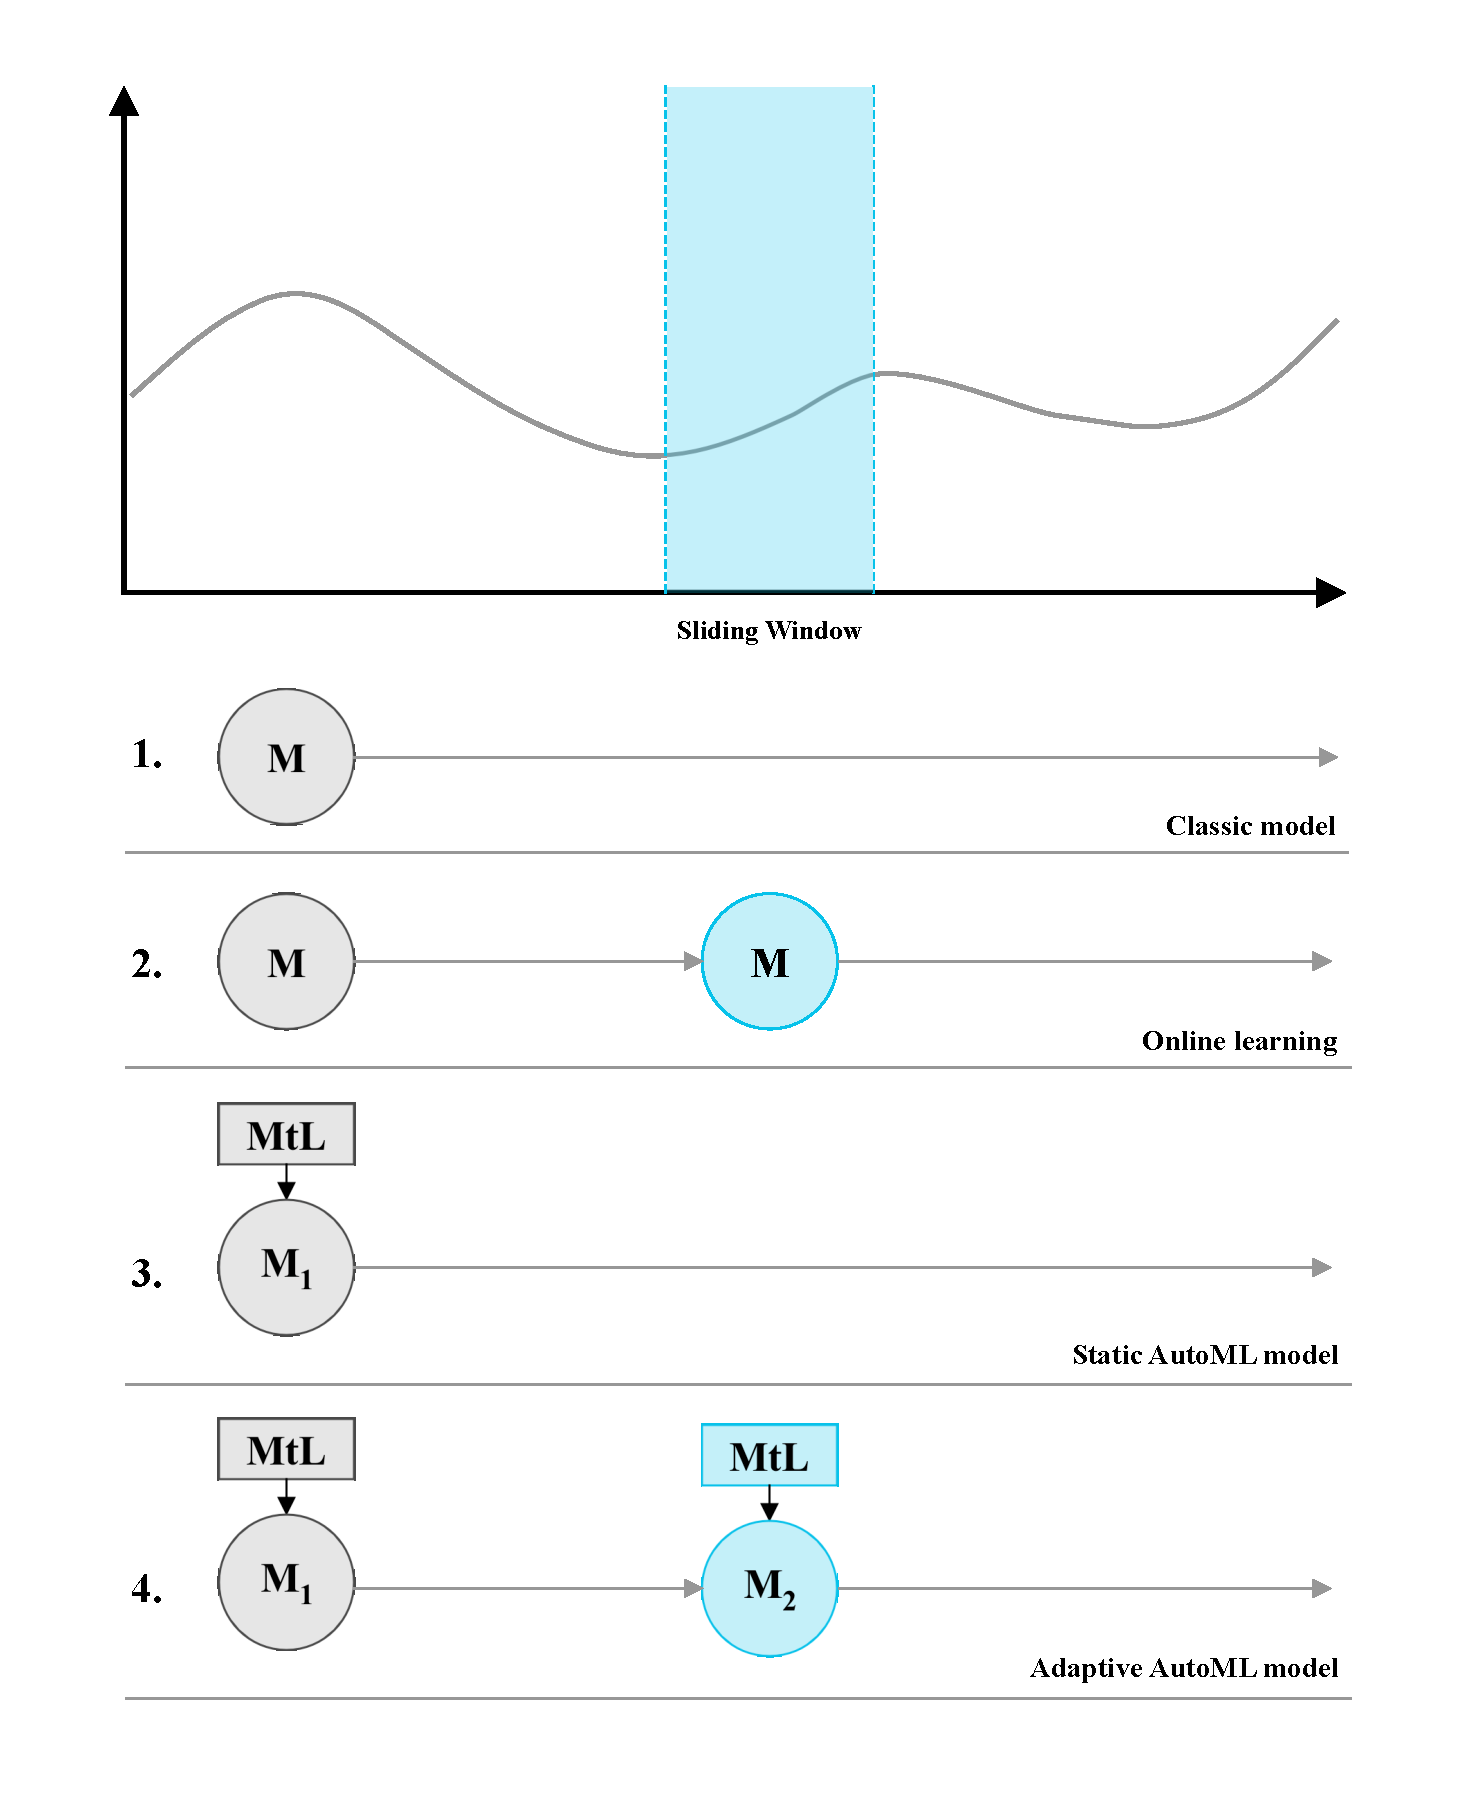
\epsfig{file=experiments.eps, width=8.5cm}
\caption{Experiment Types}
\label{fig:experiments}
\end{figure}

A visual representation of the proposed experiments types can be observed in the Figure \ref{fig:experiments}. The first two types of experiments do not involve any AutoML approach and serve as baseline for the other experiments. While the first experiment implies the usage of a model trained on a bounded part of the stream used as training data, the second experiment implies using online learning algorithms than can perform (batch) incremental learning or ensemble of those such as \textbf{Hoeffding Tree, OzaBag, OzaBoost}. The third experiment consists of using state-of-the-art AutoML libraries to select the algorithm, its features, and hyperparameters. Last experiment involves implementing theoretically described meta-learning algorithms such as BLAST or MetaStream.

The benchmark data sets includes both real and synthetic ones. The later are generated using... In order to provide verifiability and reproducibility all the datasets are published on OpenML\footnote{\url{https://openml.org/}} and their corresponding ID from the platform can be found in the table \ref{table:datasets} To convert batch data sets into streams Kafka \footnote{\url{https://kafka.apache.org}}, a widely-used distributed and scalable Pub/Sub broker was used.

\begin{table}[h]
\label{table:datasets}
\renewcommand{\arraystretch}{1.25}
\begin{tabular}{|l|l|1|} \hline
\textbf{OpenML ID} & \textbf{Dataset Name} & \textbf{Type}  \\ \hline
- & hyperplane & generated \\ \hline
- & led & generated \\ \hline
- & rbf & generated \\ \hline
- & sea & generated \\ \hline
- & covtype & real \\ \hline
- & elec & real\\ \hline
- & pokerhand & real \\ \hline
- & weather & real \\ \hline
\end{tabular}
\caption{Datasets used for the experiments}
\end{table}

\textbf{Generated datasets}
\textbf{Real datasets}
TODO: Add per dataset discussion

\section{Experiments and results}

\subsection{Experimental setup}

\subsection{Baseline models}
\subsubsection{Batch trained}
\begin{figure}[h]
\centering 
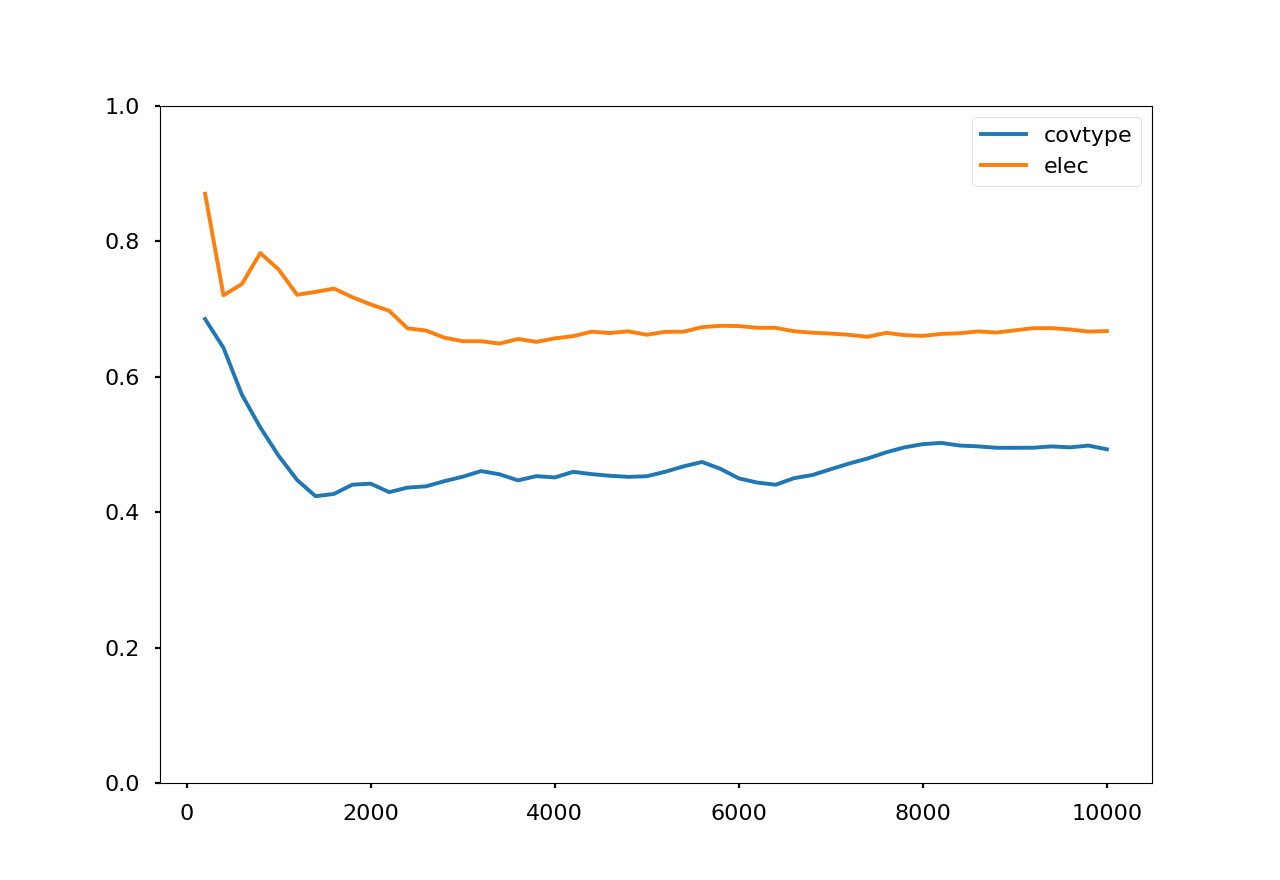
\epsfig{file=batch_LogisticRegression_all_topics.png, width=8.5cm}
\caption{Batch Logistic Regression - mean predictive accuracy for elec and covtype}
\label{fig:bathclr}
\end{figure}

\subsubsection{Online learning}

\subsection{Baseline models}
\subsubsection{Batch trained}
\begin{figure}[h]
\centering 
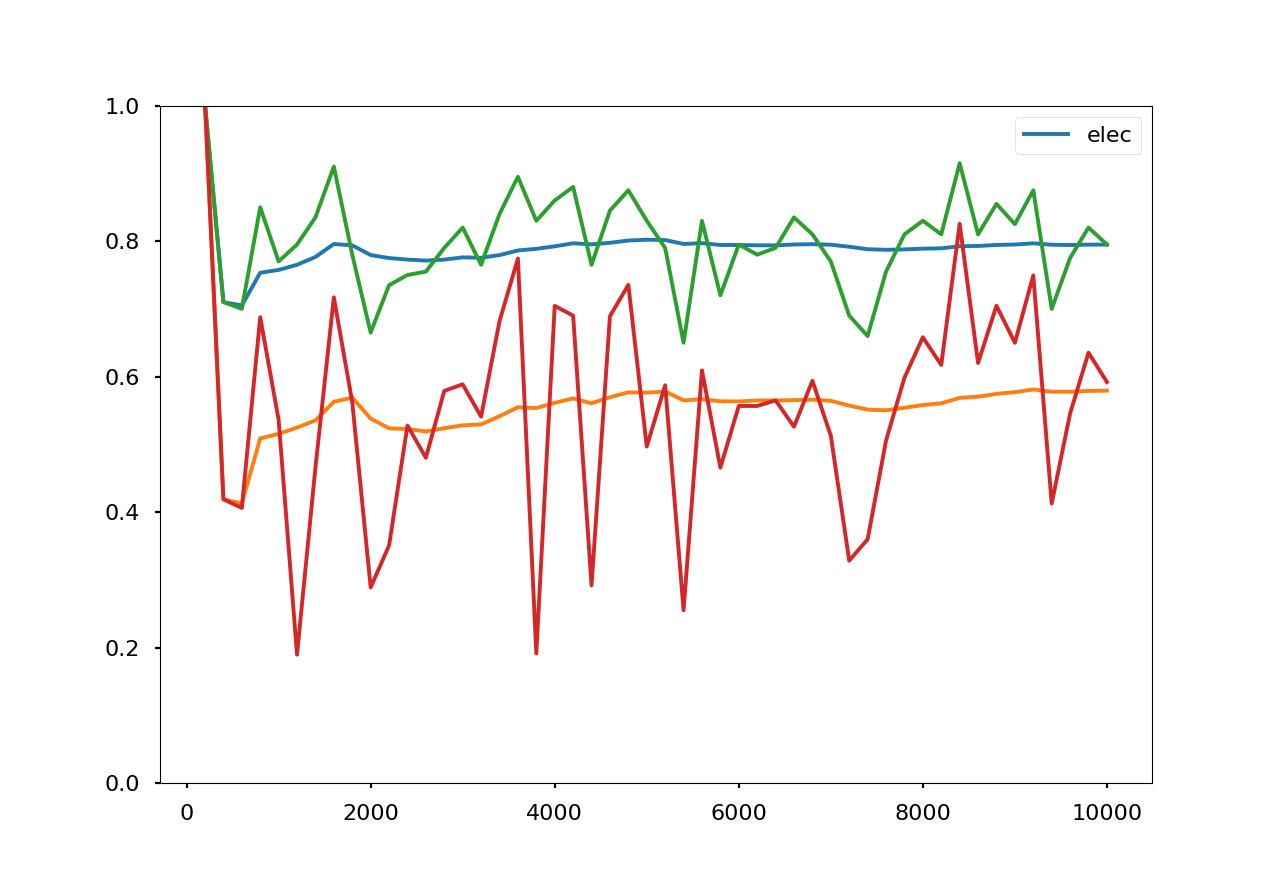
\epsfig{file=online_OzaBagging_all_topics.png, width=8.5cm}
\caption{Online OzaBagging - predictive accuracy for elec and covtype}
\label{fig:bathclr}
\end{figure}

\subsection{AutoML models}
\subsubsection{Static AutoML}
\subsubsection{Model replacement}
\subsubsection{Online meta-learning}




\section{Discussion}

- discoveries
- limitations
- contribution: automl-streams: allows implementing any algorithm, dockerized experiments, other variations

\section{Conclusion}

\section{Future Work}

% The following two commands are all you need in the
% initial runs of your .tex file to
% produce the bibliography for the citations in your paper.
\bibliographystyle{abbrv}
\bibliography{automl}  
% automl.bib is the name of the Bibliography in this case
% You must have a proper ".bib" file
%  and remember to run:
% latex bibtex latex latex
% to resolve all references
%
% ACM needs 'a single self-contained file'!


\appendix

\section{DETAILED PERFORMANCE OVER TIME}

\begin{figure*}
\centering 
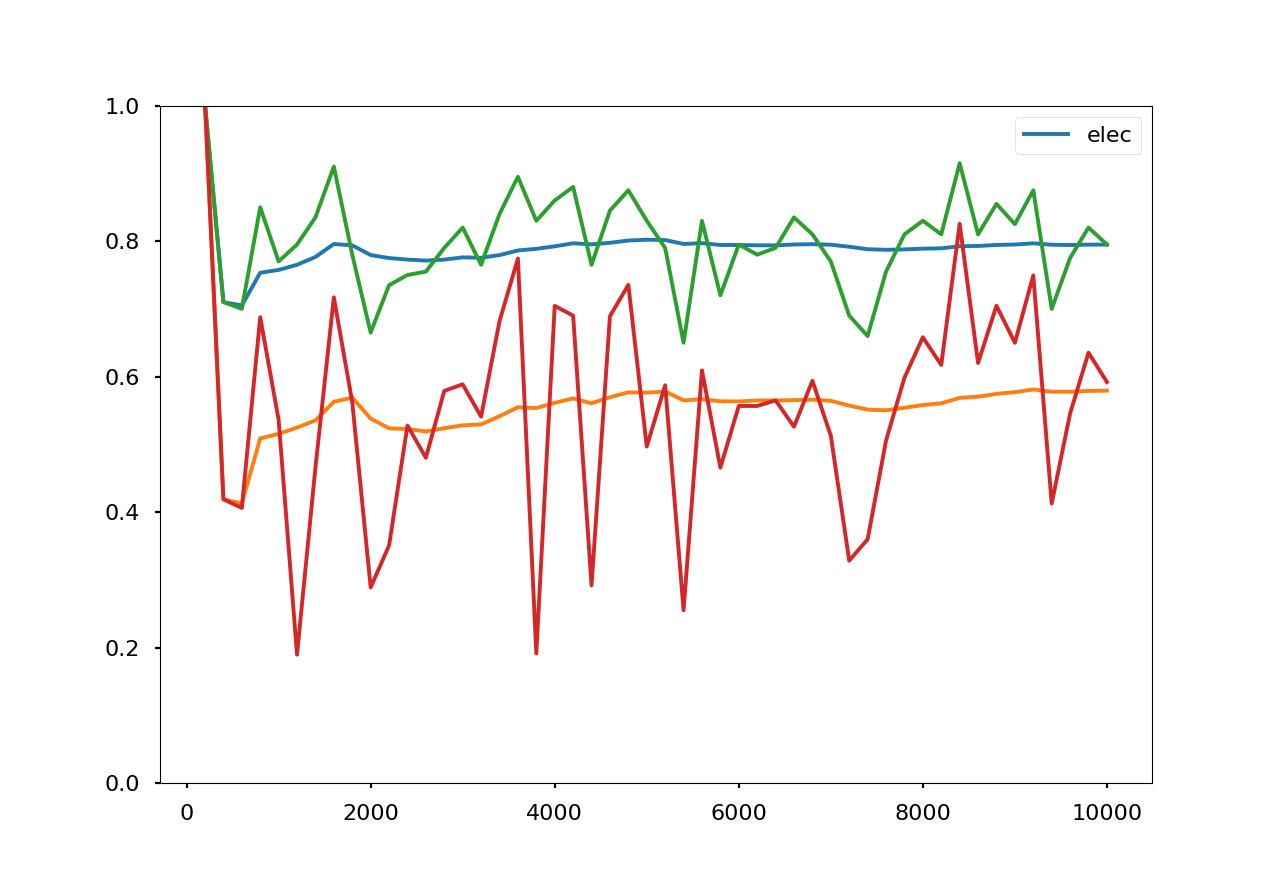
\epsfig{file=online_OzaBagging_all_topics.png, width=13cm}
\caption{Online SGD Accuracy and Kappa}
\label{fig:onlinesgd}
\end{figure*}

\end{document}
